\documentclass[11pt, oneside]{book}

%%%%%%%%%%%%%%Include Packages%%%%%%%%%%%%%%%%%%%%%%%%%%
\usepackage{xcolor}
\usepackage{mathtools}
\usepackage[a4paper, total={6in, 8in}, margin=1.25in]{geometry}
\usepackage{amsmath}
\usepackage{amssymb}
\usepackage{paralist}
\usepackage{rsfso}
\usepackage{amsthm}
\usepackage{wasysym}
\usepackage[inline]{enumitem}   
\usepackage{hyperref}
\usepackage{tocloft}
\usepackage{wrapfig}
\usepackage{titlesec}
\usepackage{colortbl}
\usepackage{stackengine} 
\usepackage{listings}
%%%%%%%%%%%%%%%%%%%%%%%%%%%%%%%%%%%%%%%%%%%%%%%%%%%%%%%%



%%%%%%%%%%%%%%%Code%%%%%%%%%%%%%%%%%%%%%%%%%%%%%%%%%%%%%
\definecolor{codegreen}{rgb}{0,0.6,0}
\definecolor{codegray}{rgb}{0.5,0.5,0.5}
\definecolor{codepurple}{rgb}{0.58,0,0.82}
\definecolor{backcolour}{rgb}{0.95,0.95,0.92}

\lstdefinestyle{mystyle}{
    backgroundcolor=\color{backcolour},   
    commentstyle=\color{codegreen},
    keywordstyle=\color{magenta},
    numberstyle=\tiny\color{codegray},
    stringstyle=\color{codepurple},
    basicstyle=\ttfamily\footnotesize,
    breakatwhitespace=false,         
    breaklines=true,                 
    captionpos=b,                    
    keepspaces=true,                 
    numbers=left,                    
    numbersep=5pt,                  
    showspaces=false,                
    showstringspaces=false,
    showtabs=false,                  
    tabsize=2
}
%%%%%%%%%%%%%%%%%%%%%%%%%%%%%%%%%%%%%%%%%%%%%%%%%%%%%%%%

%%%%%%%%%%%%%%%Chapter Setting%%%%%%%%%%%%%%%%%%%%%%%%%%
\definecolor{gray75}{gray}{0.75}
\newcommand{\hsp}{\hspace{20pt}}
\titleformat{\chapter}[hang]{\Huge\bfseries}{\thechapter\hsp\textcolor{gray75}{$\mid$}\hsp}{0pt}{\Huge\bfseries}
%%%%%%%%%%%%%%%%%%%%%%%%%%%%%%%%%%%%%%%%%%%%%%%%%%%%%%%%

%%%%%%%%%%%%%%%%%Theorem environments%%%%%%%%%%%%%%%%%%%
\newtheoremstyle{break}
  {\topsep}{\topsep}%
  {\itshape}{}%
  {\bfseries}{}%
  {\newline}{}%
\theoremstyle{break}
\theoremstyle{break}
\newtheorem{axiom}{Axiom}
\newtheorem{thm}{Theorem}[section]
\renewcommand{\thethm}{\arabic{section}.\arabic{thm}}
\newtheorem{lem}{Lemma}[thm]
\newtheorem{cor}{Corollary}[thm]
\newtheorem{defn}{Definition}[thm]
\newenvironment{indEnv}[1][Proof]
  {\proof[#1]\leftskip=1cm\rightskip=1cm}
  {\endproof}
%%%%%%%%%%%%%%%%%%%%%%%%%%%%%%%%%%%%%%%%%%%%%%%%%%%%%%


%%%%%%%%%%%%%%%%%%%%%%%Integral%%%%%%%%%%%%%%%%%%%%%%%
\def\upint{\mathchoice%
    {\mkern13mu\overline{\vphantom{\intop}\mkern7mu}\mkern-20mu}%
    {\mkern7mu\overline{\vphantom{\intop}\mkern7mu}\mkern-14mu}%
    {\mkern7mu\overline{\vphantom{\intop}\mkern7mu}\mkern-14mu}%
    {\mkern7mu\overline{\vphantom{\intop}\mkern7mu}\mkern-14mu}%
  \int}
\def\lowint{\mkern3mu\underline{\vphantom{\intop}\mkern7mu}\mkern-10mu\int}
%%%%%%%%%%%%%%%%%%%%%%%%%%%%%%%%%%%%%%%%%%%%%%%%%%%%%%



\newcommand{\R}{\mathbb{R}}
\newcommand{\N}{\mathbb{N}}
\newcommand{\Z}{\mathbb{Z}}
\newcommand{\Q}{\mathbb{Q}}
\newcommand{\C}{\mathbb{C}}
\newcommand{\T}{\mathcal{T}}
\newcommand{\M}{\mathcal{M}}
\newcommand{\Symm}{\text{Symm}}
\newcommand{\Alt}{\text{Alt}}
\newcommand{\Int}{\text{Int}}
\newcommand{\Bd}{\text{Bd}}
\newcommand{\Power}{\mathcal{P}}
\newcommand{\ee}[1]{\cdot 10^{#1}}
\newcommand{\spa}{\text{span}}
\newcommand{\sgn}{\text{sgn}}
\newcommand{\degr}{\text{deg}}
\newcommand{\pd}{\partial}
\newcommand{\that}[1]{\widetilde{#1}}
\newcommand{\lr}[1]{\left(#1\right)}
\newcommand{\vmat}[1]{\begin{vmatrix} #1 \end{vmatrix}}
\newcommand{\bmat}[1]{\begin{bmatrix} #1 \end{bmatrix}}
\newcommand{\pmat}[1]{\begin{pmatrix} #1 \end{pmatrix}}
\newcommand{\rref}{\xrightarrow{\text{row\ reduce}}}
\newcommand{\txtarrow}[1]{\xrightarrow{\text{#1}}}
\newcommand\oast{\stackMath\mathbin{\stackinset{c}{0ex}{c}{0ex}{\ast}{\Circle}}}
\newcommand{\txt}{Wald's \textit{General Relativity}}

\newcommand{\note}{\color{red}Note: \color{black}}
\newcommand{\remark}{\color{blue}Remark: \color{black}}
\newcommand{\example}{\color{green}Example: \color{black}}
\newcommand{\exercise}{\color{green}Exercise: \color{black}}

%%%%%%%%%%%%%%%%%%%%%%Roman Number%%%%%%%%%%%%%%%%%%%%%%%
\makeatletter
\newcommand*{\rom}[1]{\expandafter\@slowromancap\romannumeral #1@}
\makeatother
%%%%%%%%%%%%%%%%%%%%%%%%%%%%%%%%%%%%%%%%%%%%%%%%%%%%%%%%%

%%%%%%%%%%%%%table of contents%%%%%%%%%%%%%%%%%%%%%%%%%%%%
%\setlength{\cftchapindent}{0em}
%\cftsetindents{section}{2em}{3em}
%
%\renewcommand\cfttoctitlefont{\hfill\huge\bfseries}
%\renewcommand\cftaftertoctitle{\hfill\mbox{}}
%
%\setcounter{tocdepth}{2}
%%%%%%%%%%%%%%%%%%%%%%%%%%%%%%%%%%%%%%%%%%%%%%%%%%%%%%%%%%


%%%%%%%%%%%%%%%%%%%%%Footnotes%%%%%%%%%%%%%%%%%%%%%%%%%%%
\newcommand\blfootnote[1]{%
  \begingroup
  \renewcommand\thefootnote{}\footnote{#1}%
  \addtocounter{footnote}{-1}%
  \endgroup
}
%%%%%%%%%%%%%%%%%%%%%%%%%%%%%%%%%%%%%%%%%%%%%%%%%%%%%%%%%

%%%%%%%%%%%%%%%%%%%%%Section%%%%%%%%%%%%%%%%%%%%%%%%%%%%%
\makeatletter
\def\@seccntformat#1{%
  \expandafter\ifx\csname c@#1\endcsname\c@section\else
  \csname the#1\endcsname\quad
  \fi}
\makeatother
%%%%%%%%%%%%%%%%%%%%%%%%%%%%%%%%%%%%%%%%%%%%%%%%%%%%%%%%%

%%%%%%%%%%%%%%%%%%%%%%%%%%%%%%%%%%%Enumerate%%%%%%%%%%%%%%
\makeatletter
% This command ignores the optional argument 
% for itemize and enumerate lists
\newcommand{\inlineitem}[1][]{%
\ifnum\enit@type=\tw@
    {\descriptionlabel{#1}}
  \hspace{\labelsep}%
\else
  \ifnum\enit@type=\z@
       \refstepcounter{\@listctr}\fi
    \quad\@itemlabel\hspace{\labelsep}%
\fi}
\makeatother
\parindent=0pt
%%%%%%%%%%%%%%%%%%%%%%%%%%%%%%%%%%%%%%%%%%%%%%%%%%%%%%%%%%



\begin{document}

	\begin{titlepage}
		\begin{center}
			\vspace*{0.5cm}
			\Huge \color{red}
				\textbf{Homework 5}\\
			\vspace{0.5cm}			
			\Large \color{black}
			Physics 542 - Quantum Optics\\
			Professor Alex Kuzmich
			\vspace{1.5cm}

			
\includegraphics[scale=1.15]{hmm.pdf}
			
			
			\vspace{2cm}
			\LARGE
				\textbf{Jinyan Miao}\\
				\hfill\break
				\LARGE Fall 2023\\
			\vspace{1cm}

		\vspace*{\fill}
		\end{center}			
	\end{titlepage}

\chapter{}
\textbf{(a)} First we normalize $|\phi\rangle \sim \hat{a}|\psi\rangle$. 
\begin{align*}
|\phi\rangle = C \hat{a}|\psi\rangle\,,\qquad
\text{thus }\langle \phi | \phi\rangle = |C|^2 \langle \psi | \hat{a}^\dagger \hat{a} |\psi\rangle = |C|^2 \langle \hat{n}\rangle= 1\,,
\end{align*}
rearranging we obtain
\begin{align*}
C = \frac{1}{\sqrt{\bar{n}}}\,.
\end{align*}
Thus we write
\begin{align*}
|\phi\rangle = \frac{\hat{a}}{\sqrt{\bar{n}}}|\psi\rangle\,.
\end{align*}
Now we can compute
\begin{align*}
\langle \phi | \hat{n}|\psi\rangle &= \frac{1}{\bar{n}} \langle \psi | \hat{a}^\dagger \hat{n} \hat{a} | \psi\rangle\\ 
&= \frac{1}{\bar{n}}\langle \psi | \hat{a}^\dagger\hat{a}^\dagger \hat{a}\hat{a}|\psi\rangle \\
&= \frac{1}{\bar{n}}\langle \psi | \hat{a}^\dagger(\hat{a}\hat{a}^\dagger-1 ) \hat{a}|\psi\rangle \\
&= \frac{1}{\bar{n}}\left(
\langle \psi | \hat{a}^\dagger \hat{a}\hat{a}^\dagger\hat{a}|\psi\rangle
-
\langle \psi | \hat{a}^\dagger \hat{a}|\psi\rangle
\right) \\
&= \frac{1}{\bar{n}}\left(
\langle \psi |\hat{n}^2 |\psi\rangle -
\langle \psi | \hat{n}|\psi\rangle
\right) \\
&= \frac{1}{\bar{n}}\left(
\langle \hat{n}^2\rangle -
\bar{n}
\right) \\
&= \frac{\langle \hat{n}^2\rangle}{\langle \hat{n}\rangle} - 1\,.
\end{align*}
\textbf{(b)} Now we consider the state
\begin{align*}
|\psi\rangle = \frac{1}{\sqrt{2}}\left( |0\rangle + |10\rangle\right)\,.
\end{align*}
We first calculate
\begin{align*}
\langle \psi |\hat{n}|\psi\rangle = \frac{1}{2}\left( \langle 0 | \hat{n}|0\rangle +
\langle 10 | \hat{n}|10\rangle\right) = 5\,.
\end{align*}
Next we consider
\begin{align*}
|\phi\rangle = \frac{\hat{a}}{\sqrt{\bar{n}}} |\psi\rangle = \frac{\sqrt{10}}{\sqrt{5}\sqrt{2}}|9\rangle = |9\rangle\,.
\end{align*}
Thus we have
\begin{align*}
\langle \phi | \hat{n}|\phi\rangle = 9\,.
\end{align*}
Here we calculate
\begin{align*}
\langle \psi| \hat{n}^2 |\psi\rangle = 
\frac{1}{2}\left( \langle 0 |\hat{n}^2 |0\rangle + 
\langle 10 |\hat{n}^2|10\rangle
\right) = \frac{100}{2} = 50\,.
\end{align*}
Thus we obtain
\begin{align*}
\frac{\langle \hat{n}^2\rangle_{|\psi\rangle} }{\langle  \hat{n}\rangle_{|\psi\rangle}} - 1 = 9 = \langle \phi | \hat{n} | \phi\rangle\,
\end{align*}
as expected. The result that we find in this example is consistent with what we found in part (a). This result makes sense as $\hat{a}|0\rangle$ eliminate uncertainty on the measurement of $\hat{n}$ caused by the vacuum state $|0\rangle$. 

\chapter{}
Here we calculate
\begin{align*}
\hat{a}^\dagger |\alpha \rangle \langle \alpha | = \hat{a}^\dagger \sum_{n,m}e^{-|\alpha|^2}\frac{\alpha^n (\alpha^*)^{m}}{\sqrt{n!m!}} |n\rangle \langle m|
 = \sum_{n,m}e^{-|\alpha|^2}\frac{a^n (a^*)^{m}}{\sqrt{n!m!}}(n+1)^{1/2}|n+1\rangle \langle m|\,,
\end{align*}
On the other hand,
\begin{align*}
&\left( \alpha^* + \frac{\pd}{\pd \alpha}\right)
|\alpha \rangle \langle \alpha |\\
&{}\qquad\quad =
\alpha^* \sum_{n,m}e^{-|\alpha|^2}\frac{\alpha^n (\alpha^*)^{m}}{\sqrt{n!m!}} |n\rangle \langle m|
- \alpha^* \sum_{n,m}e^{-|\alpha|^2}\frac{\alpha^n (\alpha^*)^{m}}{\sqrt{n!m!}} |n\rangle \langle m|
+ \sum_{n,m}e^{-|\alpha|^2}\frac{n\alpha^{n-1} (\alpha^*)^{m}}{\sqrt{n!m!}} |n\rangle \langle m|\\
&{}\qquad\quad
=\sum_{n,m}e^{-|\alpha|^2}\frac{n\alpha^{n-1} (\alpha^*)^{m}}{\sqrt{n!m!}} |n\rangle \langle m|\\
&{}\qquad\quad
=\sum_{n,m}e^{-|\alpha|^2}\frac{ \alpha^{n-1} (\alpha^*)^{m}}{\sqrt{(n-1)!m!}} \sqrt{n}|n\rangle \langle m|\\
&{}\qquad\quad
=\sum_{n,m}e^{-|\alpha|^2}\frac{ \alpha^{n} (\alpha^*)^{m}}{\sqrt{n!m!}} (n+1)^{1/2}|n+1\rangle \langle m| \\
&{}\qquad\quad= \hat{a}^\dagger |\alpha \rangle \langle \alpha |\,.
\end{align*}
\newpage

For the second identity, it suffices to check it with a basis state $|n\rangle$, where we can write
\begin{align*}
|\alpha\rangle \langle \alpha | \hat{a} |n\rangle &=
\sum_{k,m}e^{-|\alpha|^2}\frac{\alpha^k (\alpha^*)^{m}}{\sqrt{k!m!}} |k\rangle \langle m| \hat{a}|n\rangle \\
&= \sum_{k,m}e^{-|\alpha|^2}\frac{\alpha^k (\alpha^*)^{m}}{\sqrt{k!m!}} |k\rangle \sqrt{n} \langle m|n-1\rangle\\
&= \sum_{k}e^{-|\alpha|^2}\frac{\alpha^k (\alpha^*)^{(n-1)}}{\sqrt{k!(n-1)!}} |k\rangle \sqrt{n} \,. 
\end{align*}
On the other hand, 
\begin{align*}
&\left( \alpha^* + \frac{\pd}{\pd \alpha}\right)
|\alpha \rangle \langle \alpha | n\rangle\\
&{}\qquad\quad =
\alpha^* \sum_{k,m}e^{-|\alpha|^2}\frac{\alpha^k (\alpha^*)^{m}}{\sqrt{k!m!}} |k\rangle \langle m|n\rangle
- \alpha \sum_{k,m}e^{-|\alpha|^2}\frac{\alpha^k (\alpha^*)^{m}}{\sqrt{k!m!}} |k\rangle \langle m|n\rangle
+ \sum_{k,m}e^{-|\alpha|^2}\frac{m\alpha^{k} (\alpha^*)^{m-1}}{\sqrt{k!m!}} |k\rangle \langle m|n\rangle\\
&{}\qquad\quad =
\sum_{k,m}e^{-|\alpha|^2}\frac{m\alpha^{k} (\alpha^*)^{m-1}}{\sqrt{k!m!}} |k\rangle \langle m|n\rangle\\
&{}\qquad\quad =
\sum_{k}e^{-|\alpha|^2}\frac{n\alpha^{k} (\alpha^*)^{n-1}}{\sqrt{k!n!}} |k\rangle \\
&{}\qquad\quad =
\sum_{k}e^{-|\alpha|^2}\frac{\alpha^{k} (\alpha^*)^{n-1}}{\sqrt{k!(n-1)!}} |k\rangle \sqrt{n} \\
&{}\qquad\quad =
|\alpha\rangle \langle \alpha | \hat{a} |n\rangle\,,
\end{align*}
which shows that 
\begin{align*}
|\alpha\rangle \langle \alpha | \,\hat{a}  = 
\left( \alpha^* + \frac{\pd}{\pd \alpha}\right)
|\alpha \rangle \langle \alpha |
\end{align*}
as $|n\rangle$ is arbitrary in the basis spanning the Hilbert space. 


\chapter{}
The state of the system is given by Eq.\,(4.120) on Gerry \& Knight, 
\begin{align*}
|\psi(t) \rangle &= \sum_{n=0}^\infty 
\left(C_eC_n \cos(\lambda t \sqrt{n+1}) - i C_g C_{n+1}\sin(\lambda t \sqrt{n+1}) \right)|e\rangle |n\rangle
\\
&{}\qquad + \sum_{n=0}^\infty \left(-i C_e C_{n-1}\sin(\lambda t\sqrt{n}) + C_gC_n \cos(\lambda t \sqrt{n})\right) |g\rangle |n\rangle
\end{align*}
We abbreviate here 
\begin{align*}
K_{e,n} &= C_eC_n \cos(\lambda t \sqrt{n+1}) - i C_g C_{n+1}\sin(\lambda t \sqrt{n+1})\,,\\
K_{g,n} &= -i C_e C_{n-1}\sin(\lambda t\sqrt{n}) + C_gC_n \cos(\lambda t \sqrt{n})\,.\\
\end{align*}
By Eq.\,(4.94) on Gerry \& Knight, we have
\begin{align*}
\hat{d} = d |g\rangle \langle e| + d^* |e\rangle \langle g|\,.
\end{align*}
Thus we have
\begin{align*}
\hat{d}|\psi(t) \rangle = 
\sum_{n=0}^\infty K_{e,n}d |g\rangle | n\rangle + K_{g,n} d^* |e\rangle |n\rangle\,.
\end{align*}
Thus we have
\begin{align*}
\langle \psi(t) |\hat{d}|\psi(t) \rangle 
&= \left(\sum_{n=0}^\infty K_{e,n}^* \langle e| \langle n| + K_{g,n}^* \langle g| \langle n| \right)\left(\sum_{n=0}^\infty K_{e,n}d |g\rangle | n\rangle + K_{g,n} d^* |e\rangle |n\rangle\right)\\
&= \left(\sum_{n=0}^\infty K_{e,n}^* \langle e| \langle n| + K_{g,n}^*  \langle g| \langle n| \right)\left(\sum_{n=0}^\infty K_{e,n}d |g\rangle | n\rangle + K_{g,n} d |e\rangle |n\rangle\right)\\
&= d\sum_{n=0}^\infty K_{e,n}^*K_{g,n}  + K_{g,n}^*K_{e,n} \,. \tag{3.1}
\end{align*}
\setcounter{equation}{1}\\
In the case where the atom is initially in excited state and the field is initially at state $|n\rangle$, we have
\begin{align*}
C_n =1\,, \qquad C_{m} = 0\text{ for }m\neq n\,,\qquad C_e = 1\,,\qquad C_g = 0\,.
\end{align*}
By comparing coefficients of terms in $K_{e,n}$ and $K_{g,n}$, we find that the products $K_{e,n}^*K_{g,n}$ and $K_{g,n}^*K_{e,n}$ always vanish in this case, thus $\langle \hat{d}\rangle = 0$. \\

On the other hand, in the semiclassical treatment of the model, we have, from Eq.\,(2.91) in Berman,
\begin{align*}
c_1 = -i \sin(\Omega t/2)\,,\qquad
c_2 = \cos(\Omega t/2)
\end{align*}
for the atom initially in excited state with exact resonance with the field. Thus we can write
\begin{align*}
|\psi(t)\rangle_{\text{semiclass.}} = -i\sin(\Omega t/2) e^{-iE_gt/\hbar}|g\rangle +\cos(\Omega t/2) e^{-i E_e t/\hbar}|e\rangle\,. 
\end{align*}
The dipole measurement in this case reads
\begin{align*}
\langle \hat{d}\rangle_{\text{semiclass.}} &= d\left(-i\cos(\Omega t/2)e^{iE_et/\hbar}\sin(\Omega t/2) e^{-iE_gt/\hbar} + i\sin(\Omega t/2) e^{iE_gt/\hbar}\cos(\Omega t/2) e^{-i E_et/\hbar} \right)\\
&= d\left(-ie^{i(E_e-E_g)t/\hbar}\cos(\Omega t/2)\sin(\Omega t/2)+ ie^{i(E_g-E_e)t/\hbar} \sin(\Omega t/2) \cos(\Omega t/2)\right)\\
&= d\left((ie^{i(E_g-E_e)t/\hbar}-ie^{i(E_e-E_g)t/\hbar})\cos(\Omega t/2)\sin(\Omega t/2)\right)\\
&= d \sin((E_e-E_g)t/\hbar) \sin(\Omega t)\,,
\end{align*}
which is non-zero for some $t >0$, thus we see that $\langle \hat{d}\rangle = 0$ in the quantum approach is purely due to the entanglement between the atom state and the field state as seen from Eq.\,(3.1). 


\chapter{}
In the case of the field initially in a coherent state, with $n \geq 0$, 
\begin{align*}
C_n = e^{-|\alpha|^2/2}\frac{\alpha^n}{\sqrt{n!}}\,.
\end{align*}
We simplify (3.1) in this text by consider the state of the atom initially in the excited state, as in the previous problems. In this case, $C_e = 1$ and $C_g = 0$, thus
\begin{align*}
K_{e,n} = e^{-|\alpha|^2/2}\frac{\alpha^n}{\sqrt{n!}}
\cos(\lambda t \sqrt{n+1})
\,,\qquad
K_{g,n} = -i e^{-|\alpha|^2/2}\frac{\alpha^{n-1}}{\sqrt{(n-1)!}}\sin(\lambda t \sqrt{n})\,.
\end{align*}
In this case (4.1) becomes
\begin{align*}
\langle \hat{d}\rangle &= 
de^{-|\alpha|^2}
\sum_{n=1}^\infty 
\frac{-2|\alpha|^{2(n-1)}\Im(\alpha)}{\sqrt{n!}\sqrt{(n-1)!} } \cos(\lambda t \sqrt{n+1})
\sin(\lambda t \sqrt{n})\\
&=
de^{-|\alpha|^2}\Im(\alpha)
\sum_{n=0}^\infty 
\frac{-2|\alpha|^{2n}}{n!\sqrt{n+1}} \cos(\lambda t \sqrt{n+2})
\sin(\lambda t \sqrt{n+1})
\end{align*}
In the case where $\alpha \in \R$, we see that $\langle \hat{d}\rangle$ vanishes, and we also observe that the sign of $\Re(\alpha)$ does not affect $\langle \hat{d}\rangle$, the sign of $\Im(\alpha)$ only flips the sign of $\langle \hat{d}\rangle$. Thus we make some plots for $\alpha \in \{1+1i, 5+1i, 1+5i, 5+5i\}$. 
\begin{center}
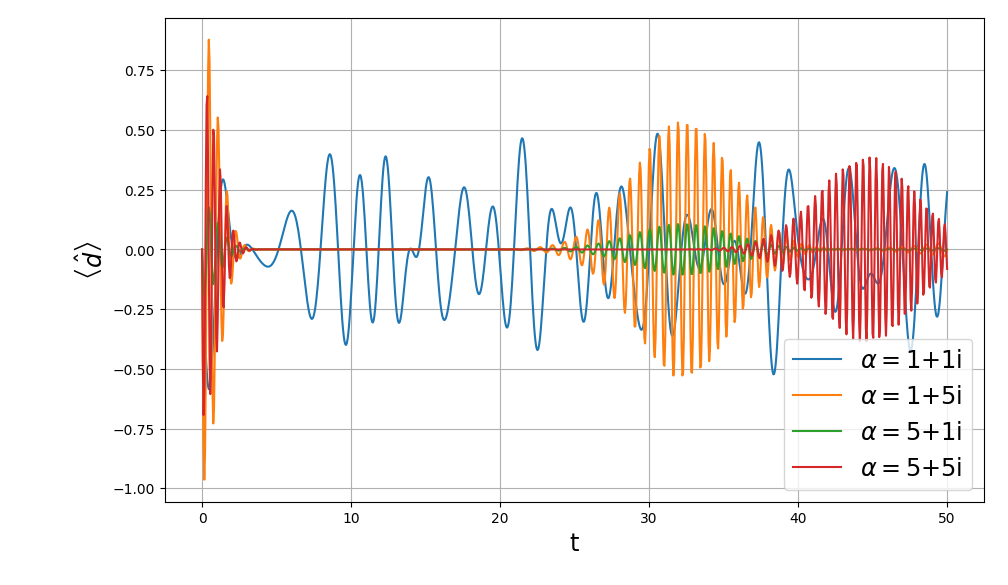
\includegraphics[scale=0.5]{542HW5/d}
\end{center}
From the figure we see that $\langle \hat{d}\rangle$ also have the collapse and recover behavior similar to that of the Rabi oscillations of the atom. While in the case of the field being in Fock state, $\langle \hat{d}\rangle$ vanishes, and in the case of semiclassical treatment of the system, $\langle \hat{d}\rangle$ oscillates periodically. 

\chapter{}
Following the analysis in Section 4.5, the inversion for field initially in a thermal state is 
\begin{align*}
W(t) = \sum_{n=0}^\infty \frac{\bar{n}^n}{(1+\bar{n})^{n+1}}  \cos(2\lambda t \sqrt{n+1})\,.
\end{align*}
Here we denote $\Omega(n) = 2\lambda \sqrt{n+1}$. The collapse time $t_c$ is estimated from the time-frequency uncertainty relation
\begin{align*}
t_c \left(\Omega(\bar{n} + \Delta n) - \Omega (\bar{n} - \Delta n)\right) \sim	 1\,.
\end{align*}
For thermal state, Eq.\,(2.149) on Gerry \& Knight gives
\begin{align*}
\Delta n = (\bar{n} + \bar{n}^2)^{1/2}\,.
\end{align*}
Thus combining, we obtain
\begin{align*}
t_c \sim \left( 
2\lambda \left(\bar{n}+1 + ( \bar{n}+\bar{n}^2 )^{1/2}\right)^{1/2} - 2\lambda \left(\bar{n}+1 - ( \bar{n}+\bar{n}^2 )^{1/2}\right)^{1/2}
\right)^{-1}\,,
\end{align*}
which gives the relation between $t_c$ and $\bar{n}$. In  the limit $\bar{n} \gg 1$, we have
\begin{align*}
t_c \sim 
\left( 
2\lambda \left(2\bar{n}\right)^{1/2} 
\right)^{-1} = \frac{1}{2\sqrt{2}\lambda \sqrt{\bar{n}}}
\end{align*}
In the limit where $\bar{n}\ll 1$, we have
\begin{align*}
t_c \sim
\left( 
2\lambda \left(1 +\bar{n}^{1/2} \right)^{1/2} - 2\lambda \left(1 - \bar{n}^{1/2}\right)^{1/2}
\right)^{-1} 
\sim
\left( 
2\lambda \left(1 + \frac{\bar{n}^{1/2}}{2} \right) - 2\lambda \left(1 - \frac{\bar{n}^{1/2}}{2}\right)
\right)^{-1} = \frac{1}{2\lambda \sqrt{\bar{n}}}\,.
\end{align*}

\chapter{}
Here we have the initial state
\begin{align*}
|\psi\rangle = \that{c}_{1,1}e^{i \omega t} e^{i\omega t/2} |1,1\rangle + \that{c}_{2,0}e^{i \omega t} e^{i\omega t/2} |2,0\rangle + 
\that{c}_{1,2}e^{i 2\omega t} e^{i\omega t/2} |1,2\rangle + \that{c}_{2,1}e^{i 2\omega t} e^{i\omega t/2} |2,1\rangle\,.
\end{align*}
Thus the probability for the atom in the excited state is 
\begin{align*}
\mathbb{P} = ||\that{c}_{2,0}||^2 + ||\that{c}_{2,1}||^2\,.
\end{align*}
From Eq.\,(15.40) in Berman, we can write
\begin{align*}
\that{c}_{2,0} = -\frac{2ig_1}{\Omega_1} \sin\left(\frac{\Omega_1t}{2}\right) \that{c}_{1,1}(0) + 
\cos\left( \frac{\Omega_1 t}{2}\right) \that{c}_{2,0}(0) = -\frac{ig}{\sqrt{2}|g|} \sin\left(|g| t\right)\,,
\end{align*}
\begin{align*}
\that{c}_{2,1} = -\frac{2ig_2}{\Omega_2} \sin\left(\frac{\Omega_2t}{2}\right) \that{c}_{1,2}(0) + 
\cos\left( \frac{\Omega_2 t}{2}\right) \that{c}_{2,1}(0) =
-\frac{ig}{\sqrt{2}|g|} \sin\left(\sqrt{2}|g|t\right)\,.
\end{align*}
WLOG, we assume here $g = -i$, then we have
\begin{align*}
\that{c}_{2,0} = -\frac{1}{\sqrt{2}} \sin(t)\,,\qquad
\that{c}_{2,0} = -\frac{1}{\sqrt{2}} \sin(\sqrt{2}t)\,.
\end{align*}
Thus the probability in the excited state is
\begin{align*}
\mathbb{P} = \frac{1}{2}\left(\sin^2(t) + \sin^2(\sqrt{2}t)\right)
\end{align*}
In order for $\mathbb{P} = 1$, we require 
\begin{align*}
t = \frac{(2n-1) \pi}{2} = \frac{(2m-1) \pi}{2\sqrt{2}} 
\end{align*}
for integers $m,n \in \Z$, thus rearranging
\begin{align*}
\sqrt{2}(2 n- 1) = 2m-1\,,
\end{align*}
while the RHS is always rational as $m \in \Q$, but the LHS is never a rational as $0\neq (2n-1) \in \Q$ and $\sqrt{2}\notin \Q$, thus such a pair $(n,m) \in \Z^2$ does not exist. We conclude that $\mathbb{P}\neq 1$. Similar reasoning holds for $\mathbb{P}\neq 0$ except at $t = 0$. The plot for $\mathbb{P}$ is attached on next page, with $g = -i/\sqrt{2}$.  

\begin{center}
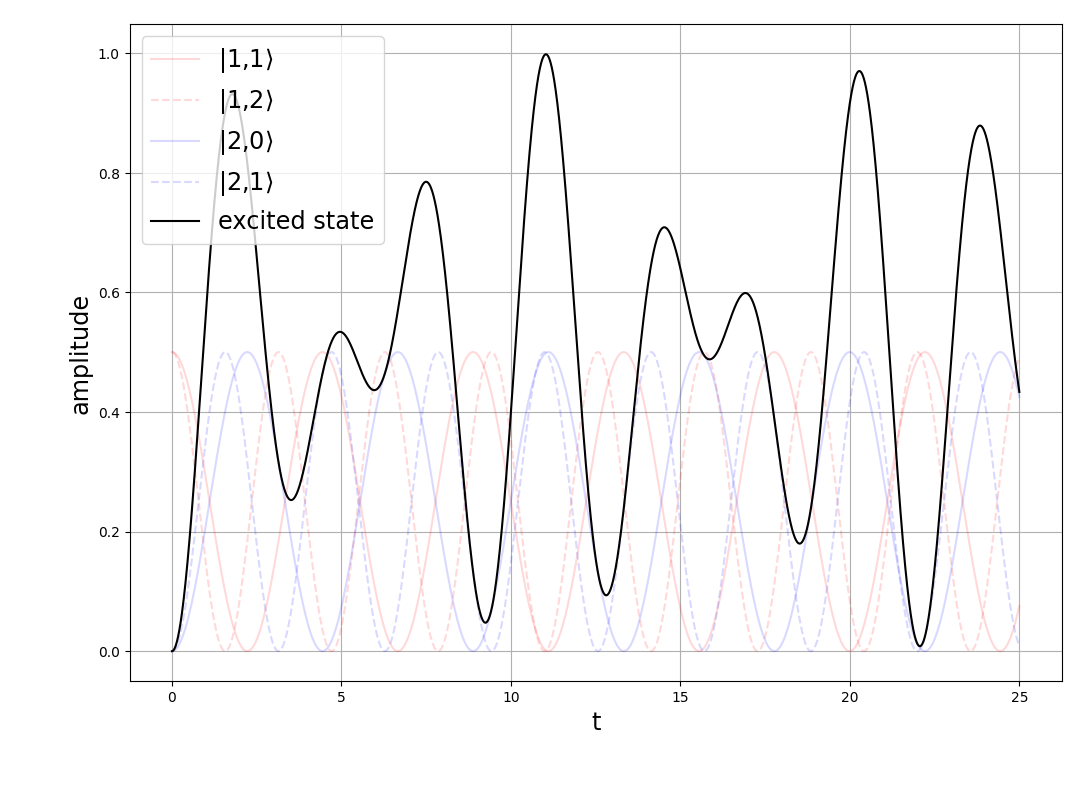
\includegraphics[scale=0.5]{542HW5/excitedState}
\end{center}
It seems like the atom reaches excited state at around $t = 11$, but in fact it is not. 
\begin{center}
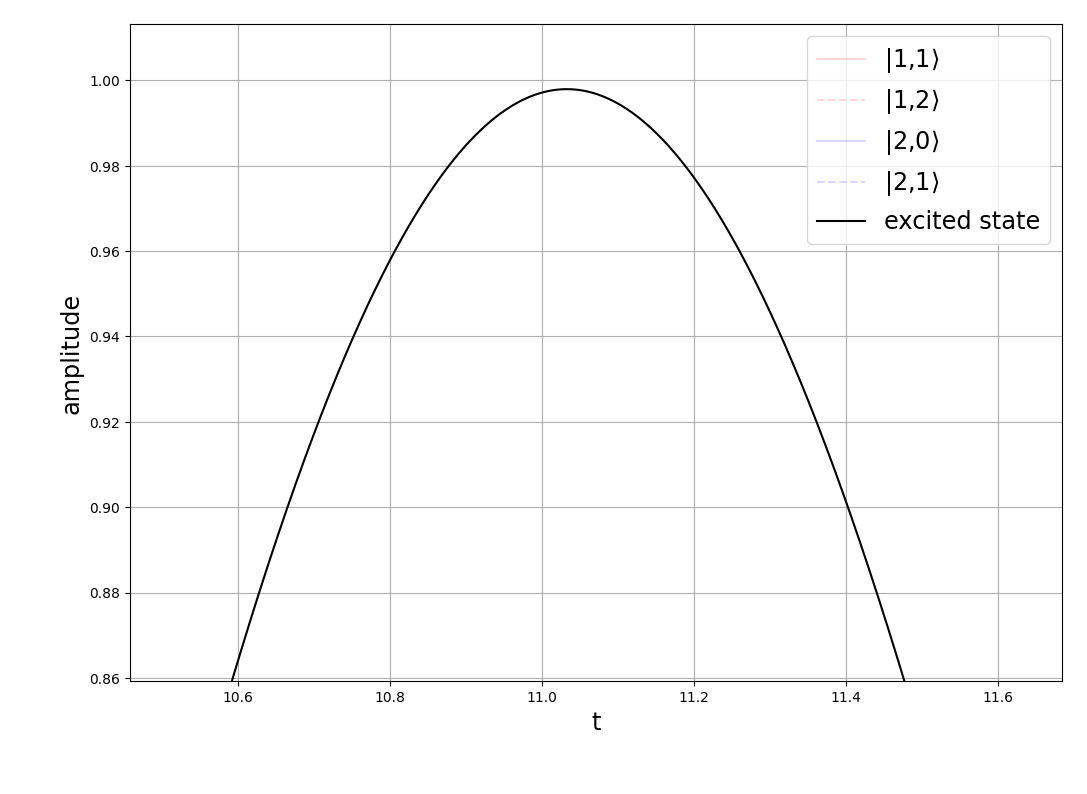
\includegraphics[scale=0.5]{542HW5/excitedStateZoomed}
\end{center}

\end{document}



